\documentclass[demonstration]{jfsma}

\usepackage[T1]{fontenc}
\usepackage{graphicx}
%\usepackage{color}
%\renewcommand\UrlFont{\color{blue}\rmfamily}
\usepackage{amsthm}
\usepackage{amsmath,amssymb,amsfonts}
\usepackage{tabularx}
\usepackage{caption}
\usepackage{listings}
% \usepackage{titlesec}
% \usepackage[english]{babel}
% \captionsetup{font=it}
\usepackage{ragged2e}
\usepackage{xurl}
\usepackage{hyperref}
\usepackage{pifont}
\usepackage{footmisc}
\usepackage{multirow}
\usepackage{enumitem}
\usepackage{algorithm2e}
\usepackage{float}
\usepackage{listings}
\usepackage{xcolor}
% \usepackage[inline, shortlabels]{enumitem}
% \usepackage[hyphens]{url}

\definecolor{codegreen}{rgb}{0,0.6,0}
\definecolor{codegray}{rgb}{0.5,0.5,0.5}
\definecolor{codepurple}{rgb}{0.58,0,0.82}
\definecolor{backcolour}{rgb}{0.95,0.95,0.92}
 
\lstdefinestyle{mystyle}{
    backgroundcolor=\color{backcolour},   
    commentstyle=\color{codegreen},
    keywordstyle=\color{magenta},
    numberstyle=\tiny\color{codegray},
    stringstyle=\color{codepurple},
    basicstyle=\footnotesize,
    breakatwhitespace=false,         
    breaklines=true,                 
    captionpos=b,                    
    keepspaces=true,                 
    numbers=left,                    
    numbersep=5pt,                  
    showspaces=false,                
    showstringspaces=false,
    showtabs=false,                  
    tabsize=2
}
 
\lstset{style=mystyle}

% --- Tickz
\usepackage{physics}
\usepackage{amsmath}
\usepackage{tikz}
\usepackage{mathdots}
\usepackage{yhmath}
\usepackage{cancel}
\usepackage{color}
\usepackage{siunitx}
\usepackage{array}
\usepackage{multirow}
\usepackage{amssymb}
\usepackage{gensymb}
\usepackage{tabularx}
\usepackage{extarrows}
\usepackage{booktabs}
\usetikzlibrary{fadings}
\usetikzlibrary{patterns}
\usetikzlibrary{shadows.blur}
\usetikzlibrary{shapes}

% ---------
% \usepackage{titlesec}
\usepackage{pdfpages}
\usepackage{booktabs}
\usepackage{csquotes}
\usepackage{lipsum}  
\usepackage{arydshln}
\usepackage{smartdiagram}
\usepackage[inkscapeformat=png]{svg}
\usepackage{textcomp}
\usepackage{tabularray}\UseTblrLibrary{varwidth}
\usepackage{xcolor}
\def\BibTeX{{\rm B\kern-.05em{\sc i\kern-.025em b}\kern-.08em
    T\kern-.1667em\lower.7ex\hbox{E}\kern-.125emX}}
\usepackage{cite}
\usepackage{amsmath}
\newcommand{\probP}{\text{I\kern-0.15em P}}
\usepackage{etoolbox}
\patchcmd{\thebibliography}{\section*{\refname}}{}{}{}

\setlength\tabcolsep{0.5pt}

\newcommand{\before}[1]{\textcolor{red}{#1}}
\newcommand{\after}[1]{\textcolor{green}{#1}}

\newcommand{\old}[1]{\textcolor{orange}{#1}}
\newcommand{\rem}[1]{\textcolor{red}{#1}}
\newcommand{\todo}[1]{\textcolor{orange}{\newline \textit{\textbf{TODO:} #1}} \newline \newline }



\newcounter{relation}
\setcounter{relation}{0}
\renewcommand{\therelation}{\arabic{relation}}
\newcommand{\relationautorefname}{Relation}

\newenvironment{relation}[1][]{%
    \refstepcounter{relation}%
    \noindent \raggedright \textit{\textbf{Relation. \therelation}} \hfill$}
{%
$ \hfill \phantom{x}

}

\newcounter{proof}
\setcounter{proof}{0}
\renewcommand{\theproof}{\arabic{proof}}
\newcommand{\proofautorefname}{Proof}

\renewenvironment{proof}[1][]{
    \refstepcounter{proof}
    \noindent \raggedright \textit{\textbf{Proof. \theproof}}

    \setlength{\leftskip}{1em}

}
{

\
\setlength{\leftskip}{0pt}
}


\titre{Une Aide à la Conception de SMA par Apprentissage par Renforcement et Modélisation Organisationnelle}


\auteur{Julien Soulé\up{a,b}}{julien.soule@lcis.grenoble-inp.fr}
\auteur{Jean-Paul Jamont\up{a}}{jean-paul.jamont@lcis.grenoble-inp.fr}
\auteur{Michel Occello\up{a}}{michel.occello@lcis.grenoble-inp.fr}
%%%Si besoin d'ajouter des auteurs à la ligne :
\auteurSuite{Louis-Marie Traonouez\up{b}}{louis-marie.traonouez@thalesgroup.com}
\auteurSuite{Paul Théron\up{c}}{paul.theron@orange.fr}

\institution{\up{a}%
  Univ. Grenoble Alpes, Grenoble INP, LCIS, 26000, Valence, France}
\institution{\up{b}%
  Thales Land and Air Systems, BU IAS, Rennes, France}
\institution{\up{c}%
  AICA IWG, La Guillermie, Franc}

% TODO: est-ce qu'on peut utiliser "dissemination" alors que le papier AIAI n'est pas publié à proprement parler?

\begin{document}

\maketitle

\begin{resume}

  % Contexte
  La conception d'un SMA peut être vue au travers de son organisation englobant les interactions individuelles jusqu'aux stratégies collectives.
  %Il s'agit alors de chercher une organisation permettant d'atteindre l'objectif donné de façon optimale sous des contraintes organisationelles données ou de l'environnement.
  % Problème
  Une approche empirique de recherche d'une organisation adéquate sur certains environments peut s'averer coûteuse en raison de leur manque d'appréhension ou leur complexité.
  % Contribution
  PRAHOM augmente le framework de simulation PettingZoo en liant modèle organisationnel et apprentissage par renforcement. Il permet d'intégrer des contraintes organisationelles dans l'apprentissage des politiques et de générer des spécifications organisationnelles d'après les comportements des agents entrainés.
  Les spécifications générées peuvent guider le concepteur.
  
\end{resume}

\motscles{Organisations, Ingénierie multi-agents, Simulation multi-agents, Apprentissage multi-agents}

\bigskip

\begin{abstract}

  % Context
  The design of an MAS can be viewed through its organization encompassing individual interactions up to collective strategies.
  %It is then a question of looking for an organization allowing the given objective to be achieved optimally under given organizational or environmental constraints.
  % Issue
  An empirical approach to finding an adequate organization in certain environments can prove costly due to their lack of apprehension or their complexity.
  % Contribution
  PRAHOM augments the PettingZoo simulation framework by linking organizational model and reinforcement learning. It makes it possible to integrate organizational constraints into policy learning and to generate organizational specifications based on the behaviors of the trained agents.
  The generated specifications can guide the designer.

\end{abstract}

\keywords{Organizations, Multi-agent engineering, Multi-agent simulation, Multi-agent learning}

\section{Introduction}

% Contexte:

%% Introduire le concept de SMA de Cyberdefense en le supportant par l'AICA
% Introduire la problématique de la conception de SMA en général à partir de ce cas précis

Un agent AICA~\cite{Kott2023}
%
(\emph{Autonomous Intelligent Cyberdefense Agent}\footnote{La recherche sur les AICA a été initiée dans le cadre du groupe \emph{NATO IST-152} puis de l'\emph{AICA International Work Group} : \url{https://www.aica-iwg.org/}.})
%
doit être déployé sur un environnement en réseaux pour détecter, identifier, caracteriser des attaques, élaborer et exécuter des contre-mesures permettant de minimiser les dommages potentiels.
Un agent AICA peut être vu comme un SMA de Cyberdefense~\cite{Singh2015} où la couverture de Cyberdéfense est distribuée sur un ensemble d'agents de Cyberdéfense collaborant entre eux de façon autonome.

Cependant, sa conception se heurte au manque de connaissance des environnements de déploiement en raison de leur variété, complexité, évolutivité, manque d'appréhension, etc. ; ou en raison de contraintes temporelles, spatiales, légales limitant l'apprentissage du fonctionnement de l'environnement par le concepteur. Au delà de la Cyberdéfense, ces difficultés sont communes dans la conception d'un SMA en général.
% La flexibilité d'un SMA de Cyberdéfense renforce sa résilience en lui permettant de s'adapter continuellement aux contraintes de l'environment tout en respectant des politiques de sûreté. Les aspects organisationels sont considerés dans l'ingénierie d'un tel SMA au sein des travaux de recherche.

%% Elargir le sujet des SMAC/AICA au contexte des SMA en général
Ce problème peut être envisagé au travers de l'\textbf{organisation} du SMA que nous voyons comme l'ensemble des logiques internes des agents visualisables du point de vue individuel jusqu'au point de vue global~\cite{Picard2009}. Les mécanismes organisationels émérgents ou choisis peuvent être explicités au travers de \textbf{modèles organisationels}.
% le \textbf{support organisationel} qui explicite comment les agents coordonnent leurs activités pour atteindre de manière collaborative un objectif commun.
La conception d'un SMA devient alors la recherche d'une organisation permettant d'atteindre l'objectif donné de façon optimale sous des contraintes environnementales.

Même si les méthodes de conception telles que GAIA~\cite{Wooldridge2000,Cernuzzi2014}, ADELFE~\cite{Mefteh2015},
% MaSE~\cite{Deloach2001}, DIAMOND~\cite{Jamont2015}
ou KB-ORG~\cite{Sims2008} facilitent la recherche d'une organisation adéquate pour un environnement et un objectif donné~\cite{Mefteh2013} ; elles ne permettent pas d'automatiser totalement la recherche des logiques internes des agents (que nous appelons \textbf{politiques}) satisfaisant les exigences données tout en explicitant les mécanismes organisationnels.

Nous introduisons \emph{PRAHOM Wrapper} (Partial Relations with Agent History and Organization Model), une couche logicielle pour le framework de simulation Multi-Agent \emph{PettingZoo} qui vise à combiner un procesus MARL (Multi-Agent Reinforcement Learning) avec le modèle organisationnel $\mathcal{M}OISE^+$~\cite{Hubner2007}. Il permet de :
%
i) Entrainer les politiques des agents à atteindre un objectif donné dans un environment et en respectant d'éventuelles spécifications organisationnelles ;\quad
ii) Determiner des spécifications organisationnelles à partir en analysant le comportement des agents entrainés.

La section II résume d'abord les concepts fondamentaux sur lesquels est construit \emph{PRAHOM Wrapper}.
Ensuite, la section III donne un aperçu du positionnement de \emph{PRAHOM Wrapper} parmi les travaux existants.
Dans la section IV, nous présentons les fonctionalités et l'utilisation de \emph{PRAHOM Wrapper} au travers d'un environnement de type jeu vidéo Atari. Enfin, la section V conclut sur \emph{PRAHOM Wrapper} en discutant de ses limitations et des travaux futurs.

% ================================================== =================================================== =

\section{Concepts fondamentaux}

Nous présentons les bases du modèle organisationnel $\mathcal{M}OISE^+$ et les bases MARL sur lesquelles est construite \emph{PRAHOM Wrapper}.

\subsection{Le modèle organisationnel $\mathcal{M}OISE^+$}

$\mathcal{M}OISE^+$~\cite{Hubner2007} permet de caractériser une organisation selon trois types de spécifications :

Les \textbf{spécifications structurelles} décrivent les moyens que les agents peuvent exploiter pour atteindre un objectif. Il comprend l'ensemble des \emph{rôles}, des sous-groupes, des \emph{liens} intra-groupe et inter-groupe, des \emph{compatibilités} intra-groupe et inter-groupe, ainsi que les \emph {cardinalités} des rôles et des sous-groupes.
% Un \emph{lien} indique si deux rôles sont liés en raison de liens de connaissance, de communication ou d'autorité. Une \emph{compatibilité} indique si deux rôles peuvent être adoptés par le même agent. Les \emph{cardinalités} de rôle et de sous-groupe font respectivement référence au nombre minimal et maximal de rôles et de sous-groupes.

Les \textbf{spécifications fonctionnelles} décrivent la manière d'atteindre un objectif. Il comprend des \emph{schémas sociaux} et des \emph{ordre de préférence}.
Un \emph{schéma social} est décrit par des objectifs globaux, des étiquettes de mission avec des plans et le cardinal des agents engagés dans une mission. Un \emph{ordre de préférence} signifie qu'un agent a une préférence sociale de s'engager dans une mission spécifique parmi plusieurs possibles.

Les \textbf{spécifications déontiques} permettent de relier les spécifications fonctionnelles et structurelles à travers un ensemble de \emph{permissions} et d'\emph{obligations}.
% Une \emph{permission} signifie qu'un agent jouant le rôle $\rho_a$ est autorisé à s'engager dans la mission $m$ pour une contrainte de temps donnée $tc$. De même, une \emph{obligation} signifie qu'un agent jouant le rôle $\rho_a$ doit s'engager dans la mission $m$ pour une contrainte de temps donnée $tc$. Une contrainte de temps $tc $ spécifie un ensemble de périodes déterminant si une autorisation ou une obligation est valide.


\subsection{L'apprentissage par renforcement multi-agent}

Le MARL est un paradigme d'apprentissage automatique dans lequel les agents apprennent à prendre des décisions en interagissant avec un environnement. L’objectif est que qu'un groupe d'agents maximisent la récompense cumulée au fil du temps grâce à un processus d’essais et d’erreurs.
Cela pousse les agents à converger vers des mécanismes de coopération, des stratégies collectives, etc.

Des modèles markoviens permettent d'appliquer les techniques MARL. En tant que modèle couramment utilisé, le Dec-POMDP~\cite{Oliehoek2016} considère plusieurs agents de façon analogue à un SMA. Il s'appuie sur des processus stochastiques pour modéliser l'incertitude de l'environnement pour les changements induits par les actions, les observations reçues, mais aussi les communications. Sa fonction de récompense est commune aux agents ce qui favorise la formation d'actions orientées pour la collaboration~\cite{Beynier2013}.
% Formellement, un Dec-POMDP est un 7-tuple $(S,\{A_i\},T,R,\{\Omega_i\},O,\gamma)$ , où : $S = \{s_1, .. s_{|S|}\}$ est l''ensemble des états possibles ; $A_{i} = \{a_{1}^{i},..,a_{|A_{i}|}^{i}\}$ l'ensemble des actions possibles pour l'agent $i$ ; $T$ pour que $T(s,a,s') = \probP{(s'|s,a)}$ l'ensemble des probabilités de transition conditionnelles entre les états ; $R : S \times A \times S \rightarrow \mathbb{R}$ la fonction de récompense ; $\Omega_{i} = \{o_{1}^{i},..,o_{|\Omega_{i}|}^{i}\}$  l'ensemble d'observations pour l'agent $ag_i$ ; $O$ pour que $O(s',a,o) = \probP{(o|s',a)}$  l'ensemble des probabilités d'observation conditionnelles ; $\gamma \in [0,1]$, le facteur de remise.

Nous appelons \textbf{résoudre}/\textbf{résoudre sous-optimalement} le Dec-POMDP pour l'équipe $t$ la recherche d'une politique conjointe $\pi_{joint,i} \in \Pi_{joint}$ permettant de maximiser/dépasser un seuil de récompense cumulée sur un horizon fini.

% ================================================== =================================================== =

\section{Travaux et positionnement}

Bien que le MARL permet de converger automatiquement vers des politiques permettant d'atteindre l'objectif donné peu de travaux tentent d’aborder la question de l'explicabilité au niveau de l'organisation. Nous identifions trois catégories de travaux dont on présente un aperçu ici.

\paragraph{\textbf{Cadres pour MARL avec aspects organisationnels}}
%
Kazhdan et. al.~\cite{Kazhdan2020} présente une bibliothèque conçue pour améliorer l'explicabilité des systèmes MARL en les rapprochant de modèles symboliques.
%
Wang et. al.~\cite{Wang2020} introduit une approche MARL orientée rôles dans laquelle les rôles sont émergents et les agents ayant des rôles similaires ont tendance à partager leur apprentissage et à se spécialiser dans certaines sous-tâches.
%
Tosic et. al~\cite{Tosic2010} a proposé un cadre pour aborder la coordination dans les SMA collaboratifs en s'appuyant sur les capacités de communication des systèmes multi-agents.
%
Zheng et. al.~\cite{Zheng2018} a présenté une plateforme pour MARL qui vise à faciliter la recherche sur l'intelligence collective artificielle en fournissant un ensemble complet dde mesures d'évaluation pour comparer les performances d'algorithmes MARL.

\paragraph{\textbf{Caractérisation des stratégies collectives émergentes}}
%
Heuillet et. al.~\cite{Heuillet2022} propose une nouvelle approche pour expliquer les stratégies coopératives en utilisant les valeurs de Shapley. Les résultats expérimentaux sur les particules multiagents et les dilemmes sociaux séquentiels démontrent l'efficacité des valeurs de Shapley pour expliquer la justification des décisions prises par les agents.
%
Jacques et. al.~\cite{Jaques2019} propose un mécanisme pour parvenir à la coordination et à la communication dans MARL en récompensant les agents pour avoir une influence causale sur les actions des autres agents. Cette approche conduit à des protocoles de communication appris conduisant à un comportement collectif plus diversifié et plus performant.

\paragraph{\textbf{Adaptation du MARL pour répondre à des exigences}}
%
% Shao et. al.~\cite{Shao2022} introduit une approche reposant sur le modèle leader-follower comme un mécanisme pour améliorer les tâches coopératives multi-agents avec des caractéristiques dynamiques, visant à améliorer l'adaptabilité et la généralisation des systèmes MARL.
%
Roy et. al.~\cite{Roy2020} présente deux méthodes de régularisation de politiques visant à améliorer la coordination dans l’apprentissage par renforcement.
%
Le \emph{Specification-Guided Reinforcement Learning} vise à synthétiser les politiques de contrôle des agents autonomes en exploitant des constructions logiques formelles pour exprimer la tâche ou l'objectif. Cette approche a conduit au développement d'algorithmes améliorant la fiabilité des modèles entrainés~\cite{Bansal2022}~\cite{Jothimurugan2023}.
%
\emph{Learning from Logical Specifications} cherche à exploiter la structure compositionnelle de la spécification pour apprendre des politiques de contrôle pour des tâches complexes~\cite{Jothimurugan2021}.

Parmi les travaux considérés, aucun n'utilise spécifiquement un modèle organisationnel comme moyen général d'exprimer à la fois les politiques MARL à un niveau collectif ; et contraindre un processus MARL selon des spécifications organisationnelles. A notre connaissance, il n'existe pas de travaux pratiques utilisables pour générer des spécifications organisationelles d'un SMA atteignant un objectif donné sur un environnement et respectant d'éventuelles contraintes d'organisation additionnelles.



% ================================================== ====================================================

\section{Aperçu de \emph{PRAHOM Wrapper}}

A la base de \emph{PRAHOM Wrapper}, l'algorithme \emph{PRAHOM} est une synthèse de deux processus:

\begin{itemize}
  \item \textbf{Determiner de spécifications organisationelles} à partir des politiques des agents à un niveau collectif ou global à partir des historiques conjoints des agents. Ce processus peut utiliser des relations déjà connues entre des sous-historiques et des spécifications organisationnelles pour aider à déduire des spécifications organisationnelles. Sinon, des techniques de comparaisons de séquences, de clustering, de classification, etc. sont utilisées pour determiner des roles pour les agents. A partir de ces roles, des les autres spécifications organisationnelles peuvent être déduites.
  \item \textbf{Contraindre des politiques conjointes} à celles satisfaisant les spécifications organisationelles données. Ce processus utilise les relations connues ou inferrées entre historiques et spécifications organisationelles pour traduire des spécifications organisationelles données en contraintes. Ces contraintes determinent ce que l'agent peut, doit, ne dois pas choisir en termes d'actions quand il reçoit une observation autorisée. Cela a pour effet de contraindre l'entrainement des politiques des agents à respecter les contraintes données.
\end{itemize}

Dans le cadre du développement de l'outil de simulation CybMASDE,
\footnote{\emph{Cyberdefense Multi Agent System Developpment Environment} est un simulateur pour SMA de Cyberdéfense disponible à \url{https://github.com/julien6/CybMASDE}}
\emph{PRAHOM PettingZoo Wrapper}\label{PettingZoo-wrapper} a été developpé comme un outil pour utiliser \emph{PRAHOM} sur un environnement PettingZoo donné. PettingZoo est une bibliothèque qui propose une API standardisée qui simplifie le développement d'environnements avec des agents et facilite l'application des algorithmes MARL.

Il s'agit d'une Preuve de Concept qui vise à lier les historiques conjointe aux spécifications $\mathcal{M}OISE^+$. Au travers d'un cas d'étude, nous proposons de présenter les fonctions pour extraire les spécifications organisationnelles brutes sous-optimales résultantes. De même lors de l'entrainement, nous présentons l'intégration des contraintes sur les observations reçus et les actions prises.

\subsection{Environnement simple : Les déménageurs}

Nous avons developpé l'environnement de type jeu Atari \emph{Moving Company} où des agents déménageurs doivent collaborer pour déplacer un paquet d'une case départ à une case finale. Pour cela les agents peuvent se déplacer sur une grille de taille, prendre et déposer le paquet sur une zone de drop. Un aperçu de l'environnement est donné en \autoref{fig:env_moving_company}.

\begin{figure}[h!]
  \centering
  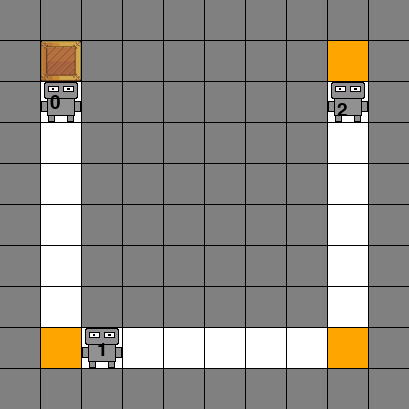
\includegraphics[width=0.15\textwidth]{figures/moving_company_1.png}
  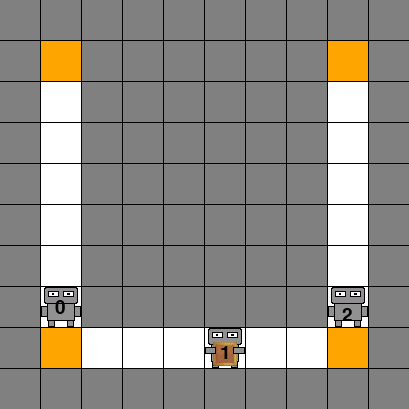
\includegraphics[width=0.15\textwidth]{figures/moving_company_2.png}
  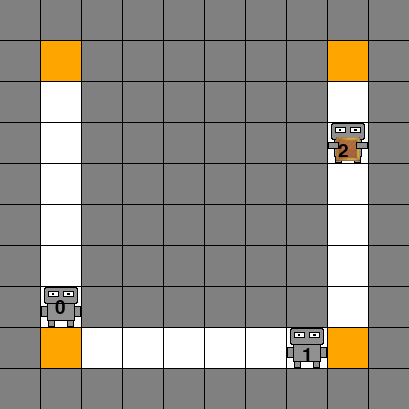
\includegraphics[width=0.15\textwidth]{figures/moving_company_3.png}
  \caption{\emph{Moving Company} avec trois agents déménageurs et un paquet à déplacer.}
  \label{fig:env_moving_company}
\end{figure}

\subsection{Utilisation de \emph{PRAHOM PettingZoo Wrapper}}

Dans \autoref{lst:wrapper_basic_use}, nous avons détaillé une utilisation basique du wrapper pour augmenter l'environnement \emph{Moving Company} (ligne 12) avec des relations connues entre les actions et les spécifications organisationnelles (ligne 4) et les contraintes de conception que les agents doivent satisfaire (ligne 8). Après l'entrainement, nous pouvons afficher une Analyse en Composantes Principales (ACP) de l'historique de chaque agent sur un épisode (ligne 14) qui est un outil d'analyse supplémentaire pour détecter manuellement les rôles émergents. Il fournit également les spécifications $\mathcal{M}OISE^+$ déduites en tenant compte des derniers épisodes et de la manière dont les agents sont instanciés dans le dernier épisode.

Ces résultats sont construits via des approches empiriques ou statistiques en utilisant les relations connues entre les observations, les actions et les spécifications organisationnelles. Lorsqu'aucune relation n'est disponible, il tente de détecter des sous-séquences d'historiques communes susceptibles de correspondre à une spécification organisationnelle (ligne 12). En raison de ces limitations, les résultats peuvent ne pas décrire entièrement l’organisation sous-jacente ou contenir des spécifications organisationnelles déduites bruyantes. Puisque les résultats sont conformes à $\mathcal{M}OISE^+$, il est alors possible de les utiliser avec les méthodes de conception SMA disponibles pour bénéficier des spécifications organisationnelles émergentes identifiées au cours du processus de conception.

\begin{lstlisting}[language=Python, caption={Utilisation basique de \emph{PRAHOM PettingZoo Wrapper}}, label={lst:wrapper_basic_use}]
from omarl_experiments import PrahomWrapper
env = PettingZoo_env.parallel_env(render_mode="human")
...
action_to_specs = {"agent_name": {
        "14": "role='leader';link='(agent_0,agent_1,auth);..."
        ...}    
    ...}
training_specs = {
    "leadadversary_0": {
        "must": ["(23,41)"],
        "must_not": ["(14,74)"]}...}
env = PrahomWrapper(env, action_to_specs, training_specs, unknown_specs_inference=True, pca_output=True)
# ...TRAINING...
env.prahom_render_pca()
trained_specs, agent_to_specs = env.prahom_specs()
\end{lstlisting}

% =============

% \begin{itemize}
% \item Questions au niveau du système multi-agents (approche centrée sur le système)
% \begin{itemize}
% \item Nombre d'agents, quelle hétérogénéité ?
% \item Quel est le support commun (Environnement) partagé par les agents ?
% \item Quels mécanismes de communication sont disponibles pour les agents ?
% \item Quels sont les langages de communication, les ontologies, les protocoles d'interaction utilisés par les agents ?
% \item Quelle est l’organisation au sein de laquelle les agents opèrent ? Comment est-il établi ?
% \item Comment les agents coordonnent-ils leurs actions ? Comment assurer un fonctionnement cohérent ?
% \end{itemize}

% \item Questions au niveau de l'agent (approche centrée sur l'agent)
% \begin{itemize}
% \item Que représente un agent ? Quelles actions doivent être encapsulées dans un agent ?
% \item Comment les agents représentent-ils l'environnement et l'organisation dans lesquels ils opèrent ?
% \item Comment les agents gèrent-ils les interactions avec d'autres agents ?
% \item Quelle est la structure interne des agents ?
% \end{itemize}
% \end{itemize}

% ================================================== =================================================== =


\section{Conclusion}

% Dans cet article, nous avons présenté AOMEA, une nouvelle approche générale de conception SMA qui vise à faciliter la conception SMA lorsqu'elle ne peut pas être facilement réalisée par les concepteurs dans des environnements de déploiement très complexes.
Les méthodes multi-agents s'appuient sur les connaissances du concepteur pour concevoir une organisation SMA adaptée mais ne fournissent pas de moyens automatiques ou assistés pour déterminer les mécanismes organisationnels pertinents.
% uniquement à partir des exigences de conception et de l'objectif global.
Les techniques MARL ont été appliquées avec succès pour entrainer automatiquement des agents à atteindre un objectif donné sans caractérisation explicite des stratégies collectives émergentes.
L'originalité d'AOMEA est d'enrichir un processus MARL d'un modèle organisationnel explicite vers un objectif méthodologique pour aborder ces problématiques. Nous avons d'abord exposé comment AOMEA est destiné à être utilisé dans l'ingénierie SMA en tant qu'outil supplémentaire pour aider au processus de conception.
Ensuite, nous avons proposé de lier les politiques des agents (modélisées dans un Dec-POMDP) avec $\mathcal{M}OISE^+$ à travers le processus \emph{PRAHOM} qui est au coeur d'AOMEA. Sous les conditions simplificatrices d'un groupe et d'un schéma social unique, \emph{PRAHOM} permet de déterminer partiellement les spécifications organisationnelles à partir des historiques conjoints et de contraindre l'entraînement des politiques par rapport à des spécifications organisationnelles.
De plus, nous avons implémenté le wrapper \emph{PRAHOM PettingZoo} comme preuve de concept pour appliquer pratiquement AOMEA et nous avons montré qu'il permet d'obtenir des spécifications organisationnelles qui satisfont aux contraintes de conception et permettent d'atteindre l'objectif donné.
Enfin, nous avons appliqué notre approche dans quatre environnements PettingZoo pour évaluer l'impact pendant et après l'entrainement. Les performances obtenus se révèlent comparables à ceux connus.

Même si \emph{PRAHOM} est agnostique à l'égard de l'algorithme MARL car il utilise l'historique des agents pour déduire des spécifications organisationnelles, reconstruire a posteriori les comportements collectifs des agents peut s'avérer difficile. En effet, une perspective majeure pour améliorer \emph{PRAHOM} est d'aller plus loin avec les techniques d'apprentissage supervisé et non supervisé en plus des approches statistiques empiriques pour identifier des spécifications organisationnelles pertinentes à partir d'historiques conjointes. De plus, il vaut la peine d’étudier les travaux récents sur les techniques MARL telles que l’apprentissage hiérarchique car ils cherchent  à caractériser les stratégies émergentes tout au long de l’apprentissage.
%À terme, nous visons également à améliorer l'applicabilité d'AOMEA en développant des interfaces dédiées construites autour de \emph{PRAHOM} le rendant plus accessible aux contextes industriels et de recherche.


% \begin{thebibliography}{9}
% {\small
% \bibitem{bar} U. Nexpert, \emph{Le livre,} Son Editeur, 1929.

% \bibitem{foo} I. Troiseu-Pami, Un article intéressant, \emph{Journal de
%     Spirou}, Vol. 17, pp. 1-100, 1987
% }
% \end{thebibliography}
\section*{Remerciements}

Ce travail est financé par Thales Land Air Systems dans le cadre des travaux conjoints de la chair Cyb'Air et de l'AICA IWG.

\section*{References}
\small
\bibliographystyle{plain}
\bibliography{references}


\end{document}

%%% Local Variables: 
%%% mode: latex
%%% TeX-SMAter: "jfsmaLatex"
%%% ispell-local-dictionary: "francais"
%%% TeX-command-extra-options: "-shell-escape"
%%% End: 